\documentclass{standalone}
\usepackage{tikz}
\usetikzlibrary{decorations.pathreplacing}
\usepackage{amsfonts}


\begin{document}
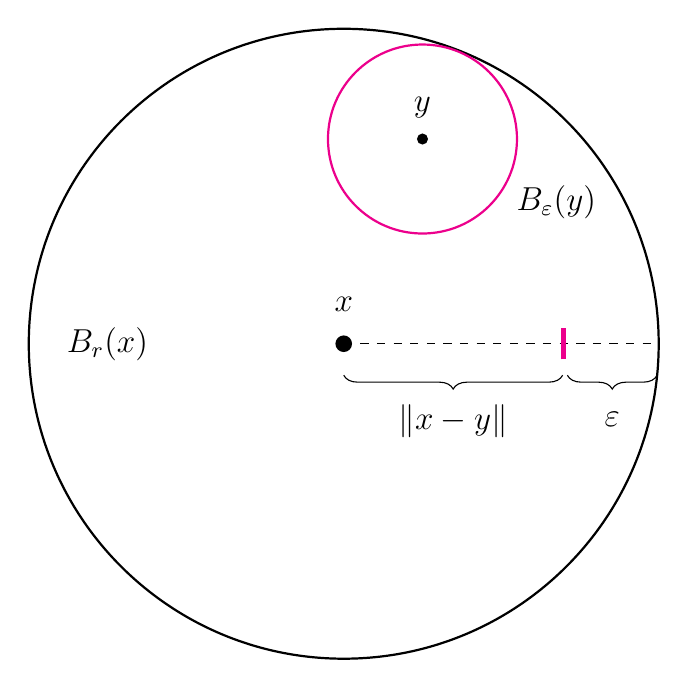
\begin{tikzpicture}
  % Draw the ellipse A
  \draw[thick] (0,0) circle (4cm);

  \node at (-3,0) {\large$B_r(x)$};
  \fill (0,0) circle (3pt);
  \node at (0,0.5) {\large$x$};
  
  % Center of the ball x
  \fill (1,2.6) circle (2pt);
  \node at (1,3) {\large$y$};
  
  % Draw the ball B_r(x)
  \draw[magenta, thick] (1,2.6) circle (1.2cm);
  \node at (2.7,1.8) {\large$B_{\varepsilon}(y)$};
  
  \draw[dashed] (0,0)--(4,0);

  
  \draw[thick, magenta, line width = 2pt] (2.79,-0.2)--(2.79,0.2);
  
\draw[decorate,decoration={brace,mirror,amplitude=5pt}] (0,-0.4) -- (2.78,-0.4) node[midway,below=7pt] {\large$\|x - y\|$};


\draw[decorate,decoration={brace,mirror,amplitude=5pt}] (2.84,-0.4) -- (3.98,-0.4) node[midway,below=10pt] {\large$\varepsilon$};
  
  
\end{tikzpicture}
\end{document}
